\documentclass[10pt,letterpaper]{article}
\usepackage[margin=0.75in,headheight=15pt]{geometry}
\usepackage[T1]{fontenc}
\usepackage{lmodern}
\usepackage{amsmath,amssymb,booktabs,graphicx,float,array}
\usepackage[font=small,labelfont=bf]{caption}
\usepackage{xcolor,fancyhdr}
\usepackage[hidelinks]{hyperref}
\usepackage{xurl}
\definecolor{navy}{RGB}{23,62,99}
\pagestyle{fancy}
\fancyhf{}
\fancyhead[L]{\small Panagiotis Housos \;|\; FRE 6991}
\fancyhead[R]{\small Homework 1: Volatility \& Correlation}
\fancyfoot[C]{\small\thepage}
\setlength{\parindent}{0pt}
\setlength{\parskip}{4pt}
\setlength{\tabcolsep}{6pt}
\setlength{\intextsep}{8pt}
\setlength{\textfloatsep}{8pt}
\captionsetup{skip=5pt}
\renewcommand{\arraystretch}{1.06}
\newcommand{\E}{\mathbb{E}}
\newcommand{\ones}{\mathbf{1}}
\newcommand{\file}[1]{\path{#1}}
\hypersetup{pdftitle={Homework 1: Volatility and Correlation},pdfauthor={Panagiotis Housos},pdfsubject={Asset Allocation FRE 6991, Fall 2026}}

\begin{document}
\begin{center}
{\Large\bfseries\color{navy} Homework 1: Volatility \& Correlation}\\[5pt]
{\large Asset Allocation --- FRE 6991, Fall 2026}\\[6pt]
\textbf{Panagiotis Housos} \quad NetID: \textbf{ph2606}\\
NYU Tandon School of Engineering\\[3pt]
Prepared November 3, 2026 \quad\textbullet\quad Due Sunday, November 8, 2026
\end{center}
\vspace{-3pt}

\section{Data and measurement conventions}
The assignment considers Apple (AAPL), Exxon Mobil (XOM), Pfizer (PFE), and
Consolidated Edison (ED). This report calculates their daily returns for
October 1, 2024 through October 1, 2026, inclusive; estimates 30-trading-day
rolling volatility and all six pairwise correlations; and constructs a
mean--variance efficient frontier from monthly returns.

Daily historical observations were obtained from Yahoo Finance through
\texttt{yfinance} and frozen as four raw CSV files on November 3, 2026.
The analysis uses the \textbf{adjusted close}, which accounts for splits and
cash dividends, rather than the unadjusted closing price. Yahoo's historical
pages and adjusted-close explanation are listed in the references. The
provided assignment is retained in the repository.

\begin{table}[H]
\centering
\caption{Sample boundaries and observation counts.}
\label{tab:sample}
\small
\begin{tabular}{p{0.40\linewidth}p{0.48\linewidth}}
\toprule
Item & Convention / observations \\
\midrule
Price observations per stock & 503, September 30, 2024--October 1, 2026 \\
Daily return observations per stock & 502, October 1, 2024--October 1, 2026 \\
Rolling window & 30 trading-day returns; 473 complete windows \\
Rolling window ending dates & November 11, 2024--October 1, 2026 \\
Monthly return observations per stock & 24, October 2024--September 2026 \\
Annualization factors & 252 trading days; 12 months \\
Sample standard deviations / covariance & Denominator $n-1$ (\texttt{ddof=1}) \\
\bottomrule
\end{tabular}
\end{table}

All stocks have identical trading dates, positive adjusted prices, and no
missing observations. No dates are dropped and no prices are forward-filled.
September 30, 2024 supplies the prior close needed to calculate the first
requested daily return. October 1, 2026 is included in the daily analysis;
the incomplete October 2026 month is excluded from monthly estimation.

For stock $i$, let $P^*_{i,t}$ denote its adjusted close. The simple daily return is
\begin{equation}
 r_{i,t}=\frac{P^*_{i,t}}{P^*_{i,t-1}}-1.
 \label{eq:daily}
\end{equation}
These are simple returns rather than logarithmic returns. Calculations use
unrounded decimal returns throughout. Tables explicitly report percentages,
dimensionless correlations, or covariance in squared decimal-return units.
The complete daily return series is supplied in
\file{results/daily_returns.csv}; selected rows appear on the next page.

\clearpage
\section{Daily returns}
\begin{table}[H]
\centering
\caption{First and last three daily returns (percent). The CSV contains all 502 dates.}
\label{tab:daily-preview}
\small\begin{tabular}{lrrrr}
\toprule
 & AAPL & XOM & PFE & ED \\
Date &  &  &  &  \\
\midrule
2024-10-01 & -2.9142\% & 2.3119\% & -0.9330\% & 0.9795\% \\
2024-10-02 & 0.2520\% & 1.3258\% & -0.2093\% & -0.6657\% \\
2024-10-03 & -0.4895\% & 0.8723\% & -0.9437\% & -0.4117\% \\
2026-09-29 & -2.6596\% & -0.7199\% & 0.0000\% & 0.4862\% \\
2026-09-30 & 1.0990\% & 0.8677\% & -0.6964\% & -1.0839\% \\
2026-10-01 & -0.8108\% & 0.6575\% & -1.4025\% & 1.2621\% \\
\bottomrule
\end{tabular}

\end{table}

\begin{table}[H]
\centering
\caption{Full daily-sample statistics (percent). Annualized volatility is $\sqrt{252}$ times daily sample standard deviation.}
\label{tab:daily-summary}
\resizebox{\linewidth}{!}{\begin{tabular}{lrrrr}
\toprule
 & Mean daily & Daily std. & Annualized vol. & Cumulative return \\
\midrule
AAPL & 0.09\% & 1.82\% & 28.83\% & 42.95\% \\
XOM & 0.09\% & 1.56\% & 24.81\% & 49.00\% \\
PFE & 0.03\% & 1.51\% & 23.95\% & 11.28\% \\
ED & 0.02\% & 1.17\% & 18.51\% & 6.27\% \\
\bottomrule
\end{tabular}
}
\end{table}

The cumulative return is $\prod_t(1+r_{i,t})-1$, covering the September 30,
2024 close through the October 1, 2026 close. XOM has the largest cumulative
return, 49.00\%, followed by AAPL at 42.95\%. AAPL has the greatest full-sample
daily-based annualized volatility, 28.83\%; ED has the smallest, 18.51\%.
The cumulative returns and mean daily returns measure different quantities:
the former compound the entire sample, whereas the latter are arithmetic averages.

\begin{figure}[H]
\centering
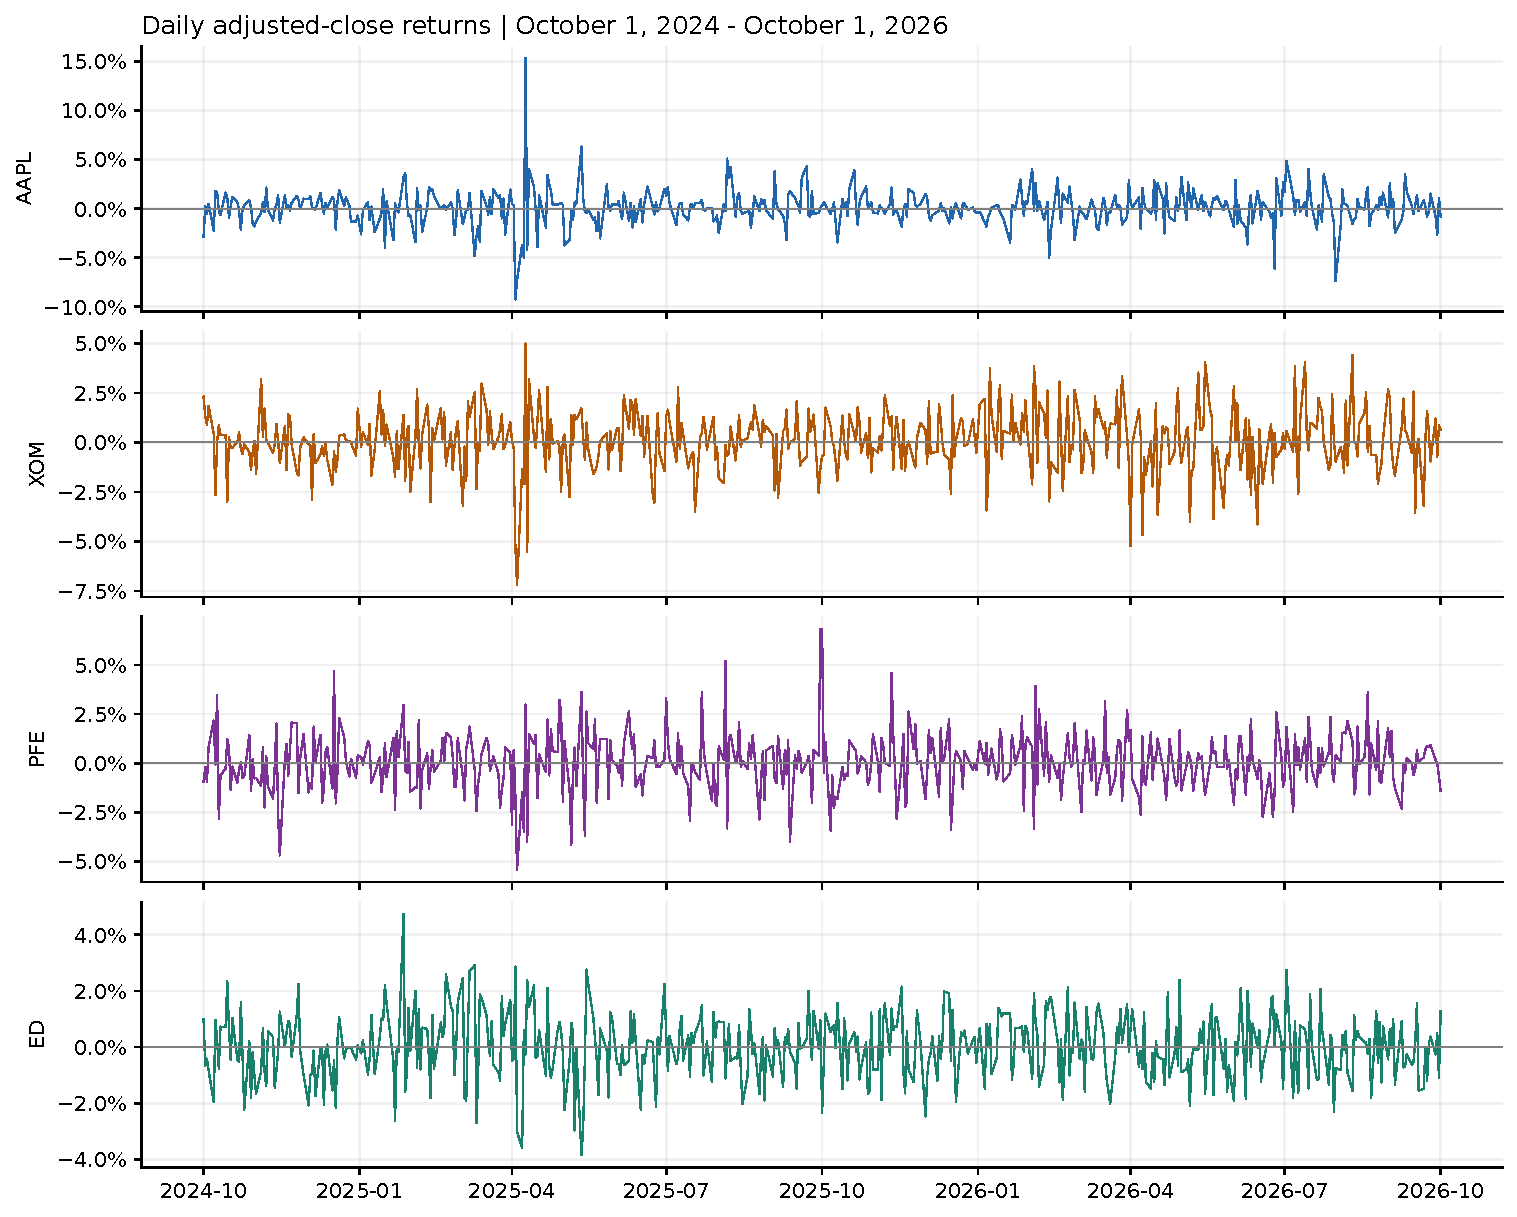
\includegraphics[width=\linewidth,height=3.5in,keepaspectratio]{../figures/daily_returns.pdf}
\caption{The four daily adjusted-close return series. The panels share dates and express returns in percent; vertical ranges vary by stock.}
\label{fig:daily}
\end{figure}

\clearpage
\section{Thirty-day rolling annualized volatility}
For each complete window ending at trading date $t$, define
\begin{equation}
 \bar r_{i,t}^{(30)}=\frac{1}{30}\sum_{k=0}^{29}r_{i,t-k},
 \qquad
 \widehat\sigma_{i,t}^{\mathrm{ann}}
 =\sqrt{252}\sqrt{\frac{1}{29}\sum_{k=0}^{29}
 \left(r_{i,t-k}-\bar r_{i,t}^{(30)}\right)^2}.
 \label{eq:vol}
\end{equation}
The window contains \textbf{30 trading days}, and advances by one trading day.
Thus there are $502-30+1=473$ volatility estimates for each stock.
The square-root-of-time conversion assumes a common daily variance scale
without serial covariance; it is a convention for comparison, not a forecast.

\begin{figure}[H]
\centering
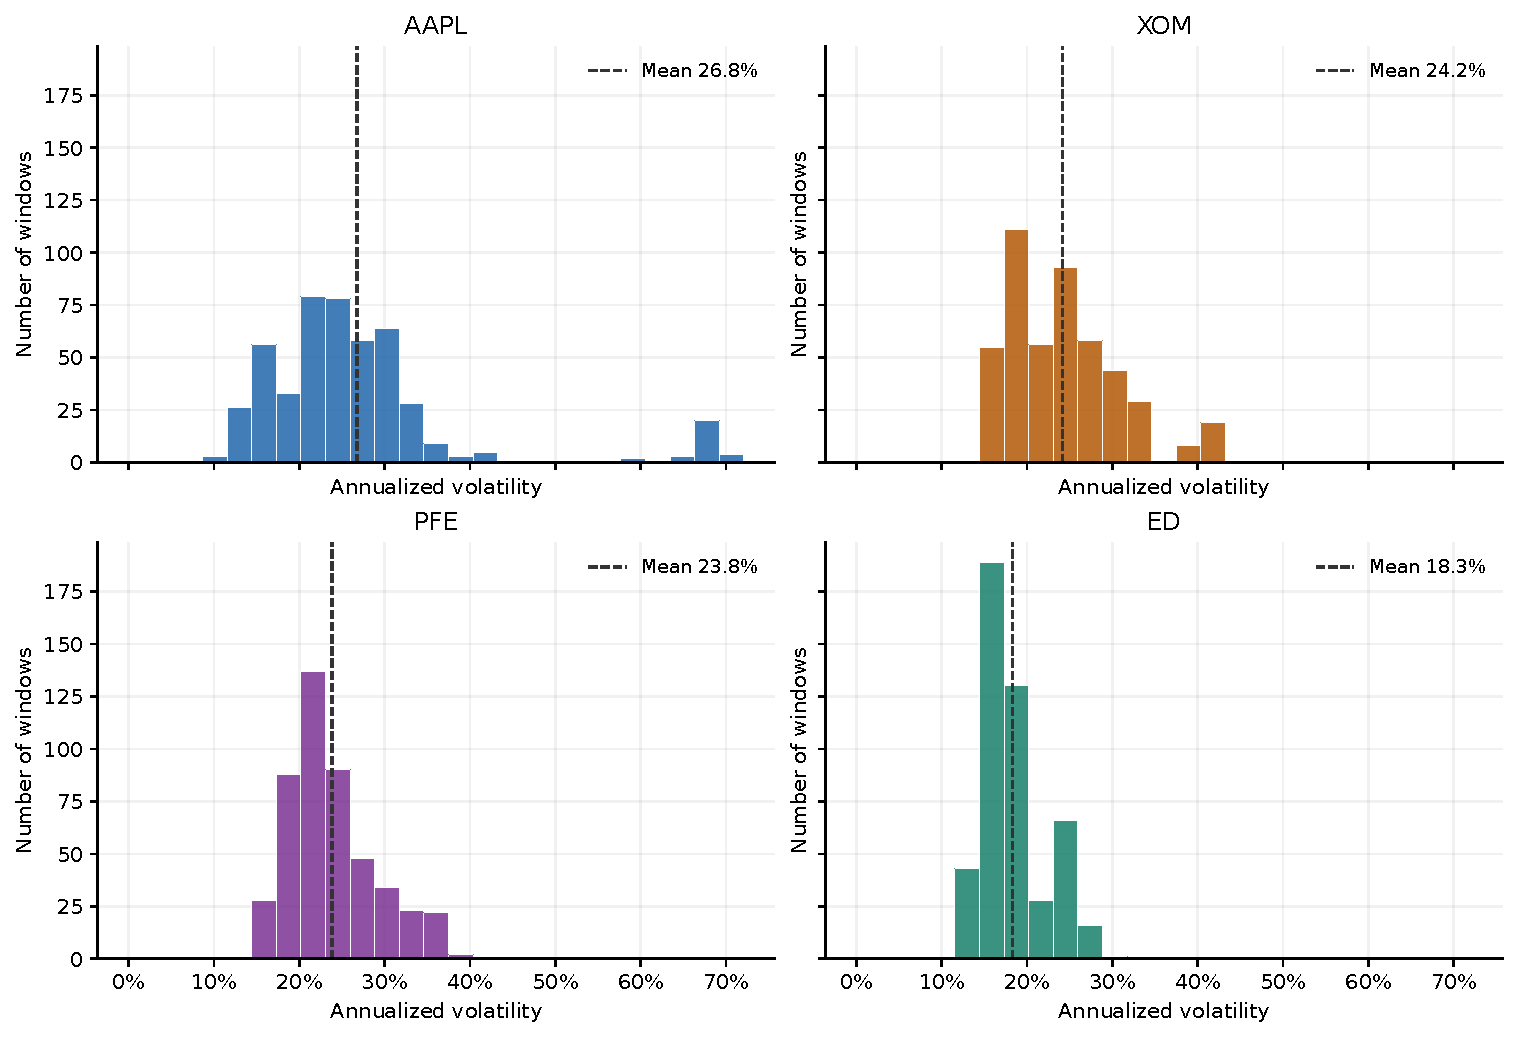
\includegraphics[width=\linewidth,height=4.1in,keepaspectratio]{../figures/volatility_histograms.pdf}
\caption{Four histograms of 30-day rolling annualized volatility, one for each stock. Common bin boundaries and axes are used. Dashed lines mark the means of the 473 estimates.}
\label{fig:vol}
\end{figure}

\begin{table}[H]
\centering
\caption{Distribution of rolling annualized volatility (percent; the standard-deviation column measures variation across windows).}
\label{tab:vol}
\small\begin{tabular}{lrrrrr}
\toprule
 & mean & std & min & median & max \\
\midrule
AAPL & 26.76\% & 12.13\% & 10.24\% & 25.11\% & 70.01\% \\
XOM & 24.19\% & 6.31\% & 14.48\% & 23.75\% & 41.77\% \\
PFE & 23.85\% & 5.09\% & 14.36\% & 22.79\% & 38.03\% \\
ED & 18.30\% & 3.63\% & 12.30\% & 17.36\% & 29.15\% \\
\bottomrule
\end{tabular}

\end{table}

AAPL's distribution has the widest spread: rolling annualized volatility
ranges from 10.24\% to 70.01\%, with a 26.76\% mean. ED has the lowest mean,
18.30\%, and the smallest standard deviation across windows, 3.63 percentage
points. XOM and PFE have similar mean rolling volatility, 24.19\% and 23.85\%.
The mean rolling volatility need not equal the full-sample volatility in
Table~\ref{tab:daily-summary}, because averaging local standard deviations
differs from taking one standard deviation over all dates.

\clearpage
\section{Thirty-day rolling correlations}
For each unordered pair $i,j$ and the same window, calculate Pearson correlation:
\begin{equation}
 \widehat\rho_{ij,t}^{(30)}=
 \frac{\sum_{k=0}^{29}(r_{i,t-k}-\bar r_{i,t}^{(30)})(r_{j,t-k}-\bar r_{j,t}^{(30)})}
 {\sqrt{\sum_{k=0}^{29}(r_{i,t-k}-\bar r_{i,t}^{(30)})^2}
  \sqrt{\sum_{k=0}^{29}(r_{j,t-k}-\bar r_{j,t}^{(30)})^2}}.
 \label{eq:corr}
\end{equation}
Correlation is dimensionless and is not annualized. There are
$\binom{4}{2}=6$ pairs and 473 estimates per pair.

\begin{figure}[H]
\centering
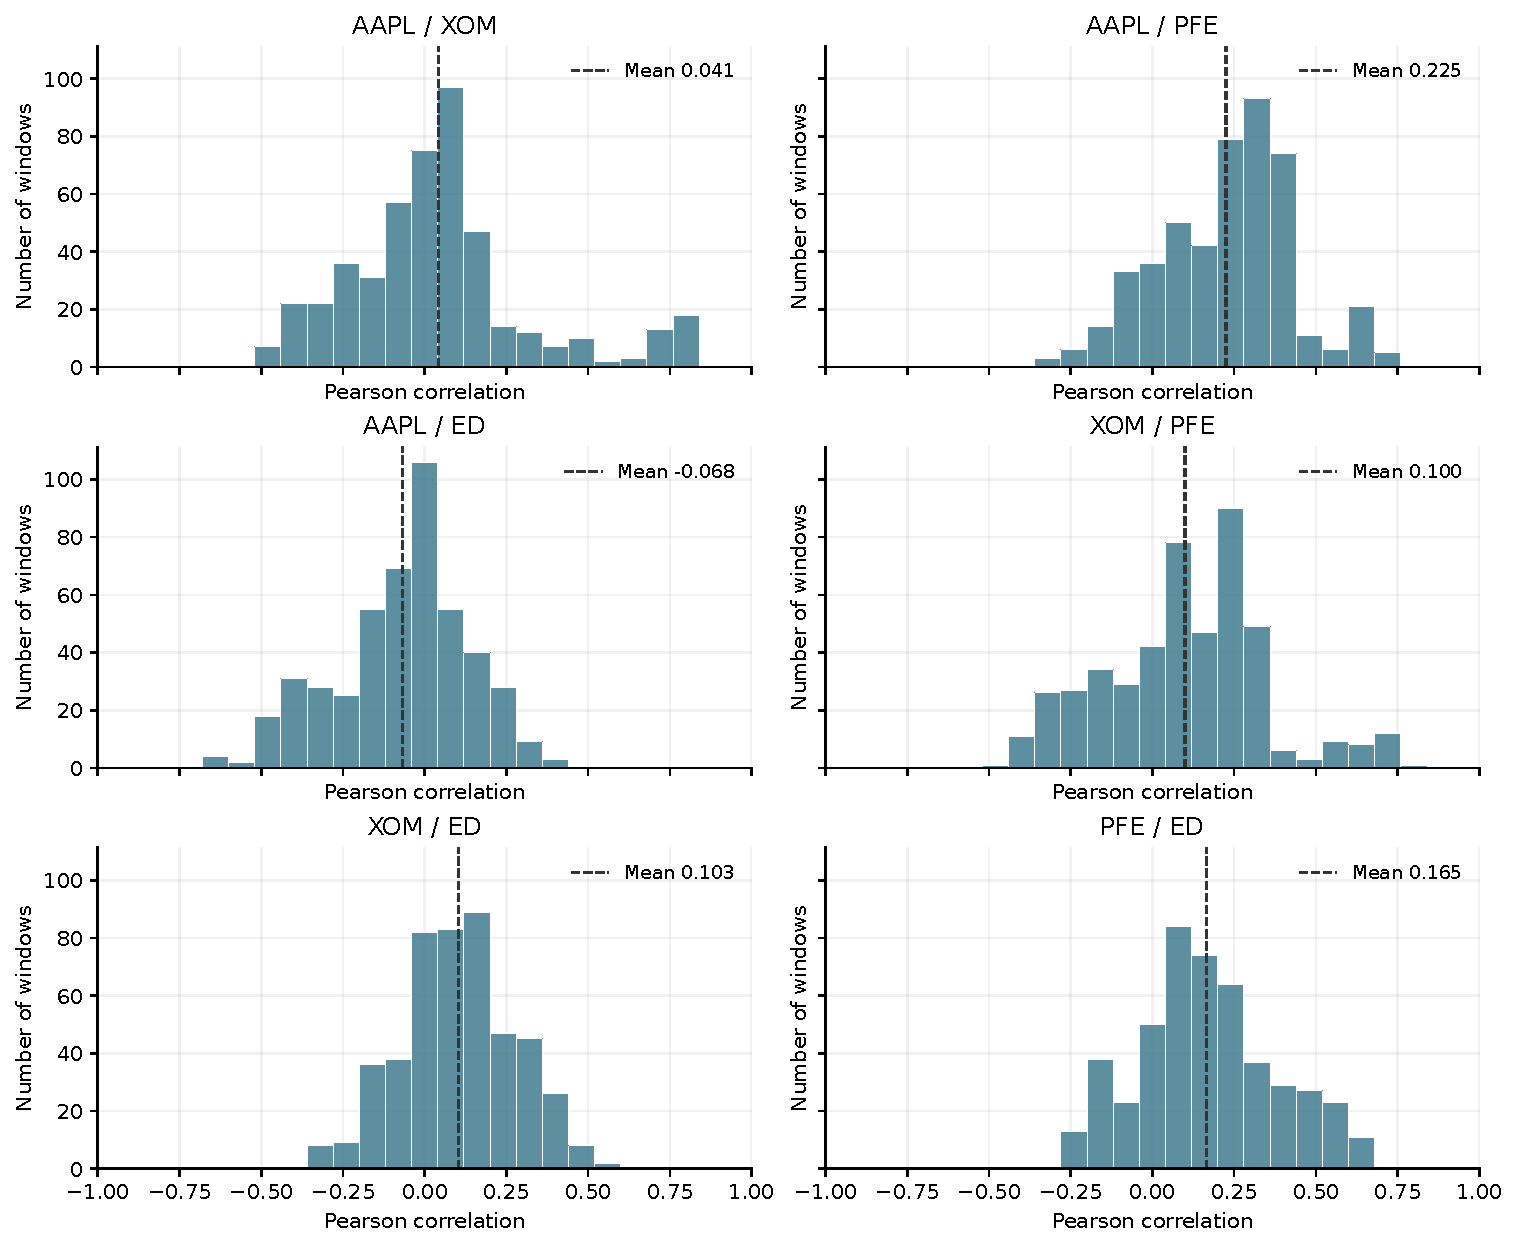
\includegraphics[width=\linewidth,height=4.5in,keepaspectratio]{../figures/correlation_histograms.pdf}
\caption{All six histograms of 30-day rolling correlations, using common bins from $-1$ to $1$. Dashed lines mark the mean correlation for each pair.}
\label{fig:corr}
\end{figure}

\begin{table}[H]
\centering
\caption{Rolling correlation summaries (dimensionless).}
\label{tab:rolling-corr}
\small\begin{tabular}{lrrrrr}
\toprule
 & mean & std & min & median & max \\
\midrule
AAPL / XOM & 0.041 & 0.279 & -0.463 & 0.032 & 0.808 \\
AAPL / PFE & 0.225 & 0.203 & -0.328 & 0.259 & 0.694 \\
AAPL / ED & -0.068 & 0.205 & -0.636 & -0.035 & 0.408 \\
XOM / PFE & 0.100 & 0.249 & -0.441 & 0.106 & 0.761 \\
XOM / ED & 0.103 & 0.174 & -0.348 & 0.102 & 0.538 \\
PFE / ED & 0.165 & 0.209 & -0.273 & 0.145 & 0.665 \\
\bottomrule
\end{tabular}

\end{table}

AAPL/PFE has the highest mean rolling correlation, 0.225. AAPL/ED is the only
pair with a negative mean, $-0.068$. All six pairs take both negative and
positive values during the sample, so a single estimate conceals substantial
variation. Adjacent windows share 29 observations: these histogram counts
describe overlapping estimates and must not be treated as independent draws.

\clearpage
\section{Monthly return statistics}
Let $P^*_{i,m}$ be the adjusted close on the last observed trading day of month
$m$. Monthly returns compound the daily returns in that month:
\begin{equation}
 R_{i,m}=\frac{P^*_{i,m}}{P^*_{i,m-1}}-1
 =\prod_{t\in m}(1+r_{i,t})-1,
 \qquad m=\text{October 2024},\ldots,\text{September 2026}.
 \label{eq:monthly}
\end{equation}
The September 30, 2024 baseline and the last trading days of the following
24 complete months give 24 monthly returns. A month-end label in the CSV can
fall on a non-trading day; the price is the last available trading-day close.
The monthly ratios were checked against compounded daily returns.

With $M=24$, the monthly arithmetic mean and sample covariance are
\begin{equation}
 \widehat\mu_{i,m}=\frac{1}{M}\sum_{m=1}^{M}R_{i,m},\qquad
 (\widehat\Sigma_m)_{ij}=\frac{1}{M-1}\sum_{m=1}^{M}
 (R_{i,m}-\widehat\mu_{i,m})(R_{j,m}-\widehat\mu_{j,m}).
\end{equation}
The frontier uses $\widehat\mu_a=12\widehat\mu_m$ and
$\widehat\Sigma_a=12\widehat\Sigma_m$, hence
$\widehat\sigma_{i,a}=\sqrt{12}\widehat\sigma_{i,m}$.
Annual means are annualized \emph{arithmetic} means, not compounded growth
rates. Covariance scaling assumes serially uncorrelated monthly returns.

\begin{table}[H]
\centering
\caption{Monthly statistics and annualized inputs from 24 monthly returns (percent).}
\label{tab:monthly}
\small\begin{tabular}{lrrrr}
\toprule
 & Monthly mean & Monthly vol. & Annual mean & Annual vol. \\
\midrule
AAPL & 1.72\% & 6.24\% & 20.60\% & 21.61\% \\
XOM & 1.88\% & 7.02\% & 22.55\% & 24.31\% \\
PFE & 0.63\% & 5.07\% & 7.51\% & 17.56\% \\
ED & 0.33\% & 5.14\% & 3.93\% & 17.79\% \\
\bottomrule
\end{tabular}

\end{table}

\begin{table}[H]
\centering
\caption{Monthly return correlation matrix (dimensionless).}
\label{tab:monthly-corr}
\small\begin{tabular}{lrrrr}
\toprule
 & AAPL & XOM & PFE & ED \\
\midrule
AAPL & 1.0000 & -0.1402 & 0.2539 & -0.4491 \\
XOM & -0.1402 & 1.0000 & 0.5059 & 0.3911 \\
PFE & 0.2539 & 0.5059 & 1.0000 & -0.0061 \\
ED & -0.4491 & 0.3911 & -0.0061 & 1.0000 \\
\bottomrule
\end{tabular}

\end{table}

\begin{table}[H]
\centering
\caption{Monthly sample covariance matrix (squared decimal-return units, not percent). Annualized covariance is this matrix multiplied by 12.}
\label{tab:monthly-cov}
\small\begin{tabular}{lrrrr}
\toprule
 & AAPL & XOM & PFE & ED \\
\midrule
AAPL & 0.003892 & -0.000614 & 0.000803 & -0.001439 \\
XOM & -0.000614 & 0.004925 & 0.001800 & 0.001410 \\
PFE & 0.000803 & 0.001800 & 0.002571 & -0.000016 \\
ED & -0.001439 & 0.001410 & -0.000016 & 0.002638 \\
\bottomrule
\end{tabular}

\end{table}

XOM has the largest annualized mean, 22.55\%, and the largest monthly-based
annualized volatility, 24.31\%. PFE has the smallest annualized volatility,
17.56\%. The strongest positive monthly correlation is XOM/PFE, 0.5059;
AAPL/ED is the most negative, $-0.4491$, and contributes diversification.
Monthly correlations and average rolling daily correlations differ because
aggregation and the estimation windows differ. These are separate estimates.

\clearpage
\section{Efficient frontier: formulation and portfolios}
The primary analysis assumes a fully invested portfolio with no short sales:
\begin{equation}
 \ones^T w=1,\qquad w_i\geq 0,\qquad
 \mu_p=w^T\widehat\mu_a,\qquad
 \sigma_p=\sqrt{w^T\widehat\Sigma_a w}.
 \label{eq:portfolio}
\end{equation}
No transaction costs, taxes, or risk-free asset are included. A risk-free
rate is not specified in the assignment, so a tangency portfolio or capital
allocation line is not calculated.

First, solve the global minimum-variance problem with the budget and
nonnegativity constraints. Then, for each target annual arithmetic return $q$
from the minimum-variance portfolio's mean through the largest asset mean,
solve
\begin{equation}
 \min_w w^T\widehat\Sigma_a w
 \quad\text{subject to}\quad
 \ones^T w=1,\quad \widehat\mu_a^T w=q,\quad w\geq 0.
 \label{eq:frontier}
\end{equation}
This upper branch is the efficient frontier: it gives the smallest volatility
available at each efficient expected return. The lower-return branch below
the minimum-variance portfolio's mean is not efficient.

\subsection*{Exact constrained solution}
With four assets, all $2^4-1=15$ possible nonempty supports can be examined.
For a support $S$, let $C_S$ be its annual covariance submatrix, and define
\begin{equation}
 H_S=\begin{pmatrix}\ones_S^T\\\widehat\mu_{a,S}^T\end{pmatrix},
 \qquad b=\begin{pmatrix}1\\q\end{pmatrix},\qquad
 w_S=C_S^{-1}H_S^T\left(H_SC_S^{-1}H_S^T\right)^{-1}b.
 \label{eq:support}
\end{equation}
Feasible nonnegative solutions are retained and their variances compared;
single-asset supports are handled directly. For the global minimum-variance
problem, $H_S=\ones_S^T$ and $b=1$. The covariance matrix is positive definite,
so this procedure finds the global constrained solution. The graph samples
201 targets; each target is solved analytically over the possible supports.
Random portfolios illustrate the feasible region, and do not determine the frontier.

\begin{table}[H]
\centering
\caption{Selected fully invested long-only portfolios. Weights, annualized arithmetic means, and annualized volatilities are percentages.}
\label{tab:portfolios}
\resizebox{\linewidth}{!}{\begin{tabular}{lrrrrrr}
\toprule
 & AAPL & XOM & PFE & ED & Annual mean & Annual vol. \\
\midrule
Minimum variance & 33.05\% & 0.00\% & 19.76\% & 47.19\% & 10.15\% & 9.59\% \\
Equal weight & 25.00\% & 25.00\% & 25.00\% & 25.00\% & 13.65\% & 11.59\% \\
Midpoint target & 46.58\% & 24.99\% & 0.00\% & 28.43\% & 16.35\% & 11.18\% \\
Maximum mean & 0.00\% & 100.00\% & 0.00\% & 0.00\% & 22.55\% & 24.31\% \\
\bottomrule
\end{tabular}
}
\end{table}

The minimum-variance allocation is \textbf{33.05\% AAPL, 0.00\% XOM,
19.76\% PFE, and 47.19\% ED}. Its estimated annual mean is 10.15\%, and
its annual volatility is 9.59\%, below the volatility of every individual stock.
The midpoint target is halfway between the minimum-variance mean and the
largest asset mean, not a portfolio with equal weights. It has 16.35\% mean
and 11.18\% volatility, compared with 13.65\% and 11.59\% for equal weights.
Thus equal weights are inefficient under these sample estimates. The highest
feasible long-only mean, 22.55\%, is obtained by holding 100\% XOM.

\clearpage
\section{Efficient frontier: graph and interpretation}
\begin{figure}[H]
\centering
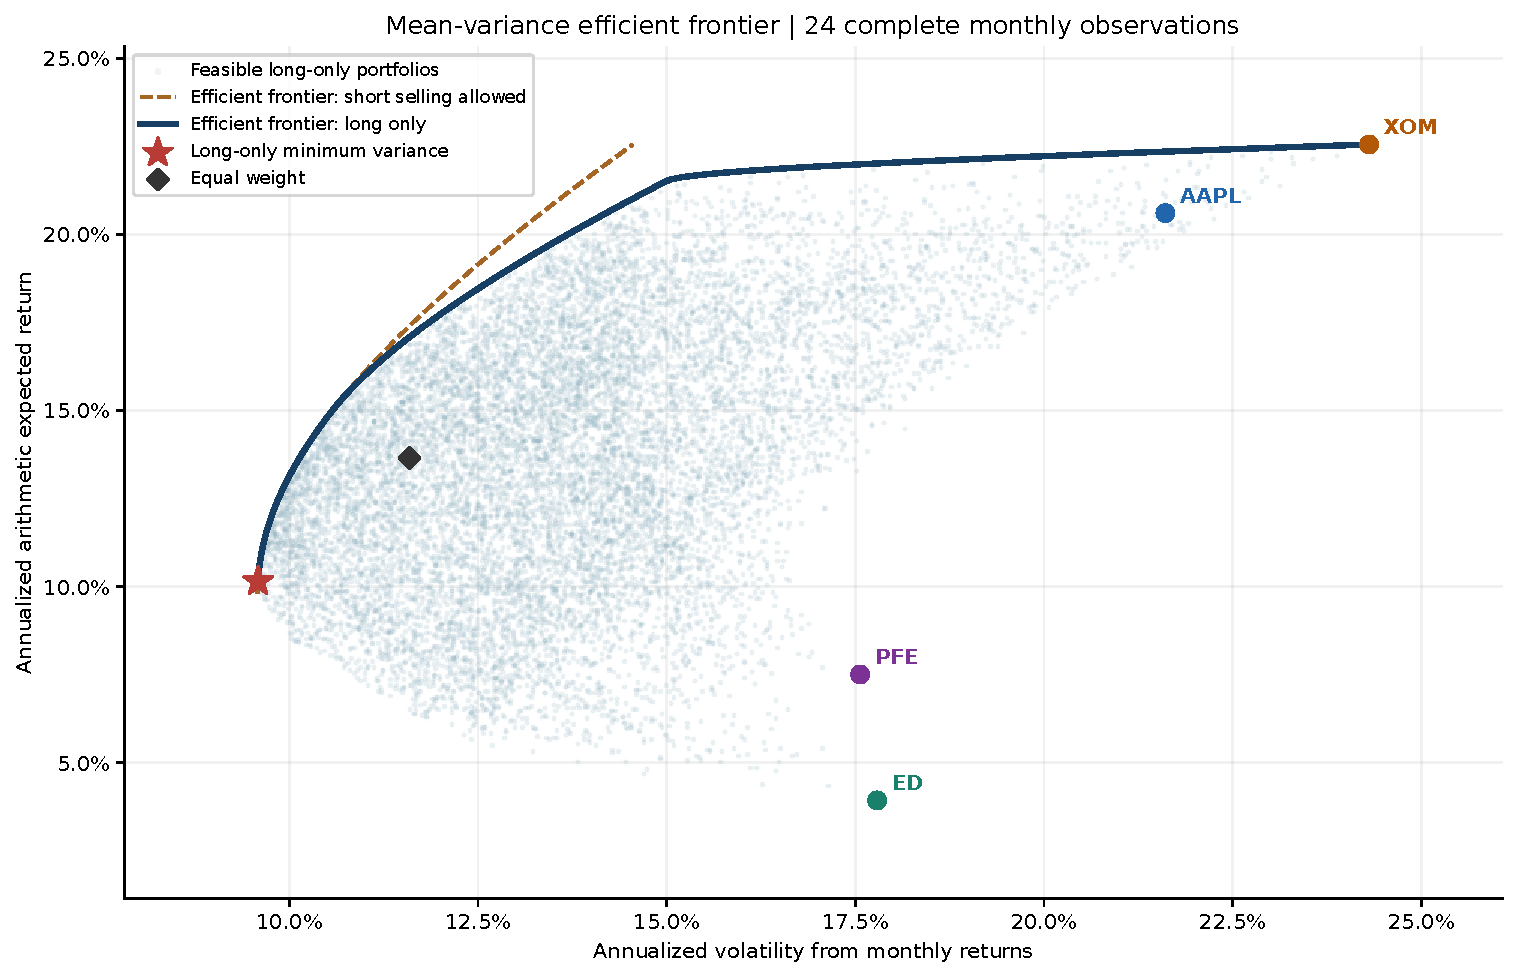
\includegraphics[width=\linewidth,height=4.2in,keepaspectratio]{../figures/efficient_frontier.pdf}
\caption{Efficient frontiers using annualized moments estimated from the 24 monthly returns. The solid line is the long-only upper frontier; the dashed line permits short sales. The cloud contains 12,000 illustrative long-only portfolios. Individual stocks, the long-only minimum-variance portfolio, and equal weights are marked.}
\label{fig:frontier}
\end{figure}

The leftmost point of the long-only frontier is the minimum-variance portfolio.
Moving upward along the curve requires increasing risk to achieve larger
estimated returns. A substantial allocation to ED can reduce portfolio
variance despite ED's low estimated mean, in part because its monthly
returns correlate negatively with AAPL. The efficient allocation changes
with the target return; minimum standalone volatility alone does not determine
portfolio weights.

\subsection*{Supplemental frontier with short selling permitted}
Removing $w\geq0$ retains the fully invested budget and target-return
constraints. Define, using the full annual covariance matrix $C=\widehat\Sigma_a$,
\begin{equation}
 a=\ones^TC^{-1}\ones,\quad
 b=\ones^TC^{-1}\widehat\mu_a,\quad
 c=\widehat\mu_a^TC^{-1}\widehat\mu_a,\quad d=ac-b^2.
\end{equation}
The unrestricted minimum variance at target $q$ is
\begin{equation}
 \sigma^2(q)=\frac{aq^2-2bq+c}{d},\qquad
 w(q)=C^{-1}\left(\frac{c-bq}{d}\ones+
                         \frac{aq-b}{d}\widehat\mu_a\right).
\end{equation}
Its efficient branch starts at $q=b/a$. The unrestricted minimum-variance
portfolio has approximately 32.75\% AAPL, $-1.83$\% XOM, 21.10\% PFE, and
47.98\% ED, with 9.81\% annual mean and 9.58\% annual volatility. Removing
nonnegativity weakly lowers minimum risk for a given feasible target.
For comparison, the dashed curve is displayed only through XOM's estimated
mean. Unrestricted feasible target returns extend beyond that displayed
range; XOM's mean is an upper bound only for long-only portfolios.

\clearpage
\section{Reproducibility and interpretation limits}
The repository includes raw data, calculation code, full-precision CSV results,
an Excel workbook, chart files, the LaTeX source, and this report. All paths
below are relative to the repository root.

\begin{table}[H]
\centering
\caption{Principal calculation artifacts. CSV returns and weights use decimals.}
\small
\begin{tabular}{>{\raggedright\arraybackslash}p{0.37\linewidth}>{\raggedright\arraybackslash}p{0.55\linewidth}}
\toprule
Artifact & Path \\
\midrule
Original assignment & \file{assignment/HW1_VOLATILITY AND CORRELATION1.docx} \\
Frozen adjusted-price source files & \file{data/raw/AAPL.csv}, \file{XOM.csv}, \file{PFE.csv}, \file{ED.csv} in the same directory \\
Download metadata & \file{data/raw/download_metadata.json} \\
Reproducible analysis & \file{scripts/analyze.py} \\
All daily returns & \file{results/daily_returns.csv} \\
All rolling volatility estimates & \file{results/rolling_30d_annualized_volatility.csv} \\
All six rolling correlations & \file{results/rolling_30d_correlations.csv} \\
Monthly returns and moments & \file{results/monthly_returns.csv}, \file{monthly_summary.csv}, \file{monthly_correlation.csv}, \file{monthly_covariance.csv} in \file{results/} \\
Annual covariance for optimization & \file{results/annualized_monthly_covariance.csv} \\
Frontier returns, risk, and weights & \file{results/efficient_frontier_long_only.csv}; \file{results/efficient_frontier_unconstrained.csv} \\
Excel calculation workbook & \file{results/homework1_calculations.xlsx} \\
Validation and source-file hashes & \file{results/summary.json} \\
\bottomrule
\end{tabular}
\end{table}

Run \texttt{python scripts/analyze.py} from the repository root after installing
the dependencies in \file{requirements.txt}. The frozen CSV inputs allow
reproduction without downloading prices again. Generated LaTeX tables and
PDF charts are read directly into this report, reducing transcription error.
Checks verify aligned dates, no missing prices, the number of rolling windows,
monthly compounding, symmetric correlations, positive-definite covariance,
portfolio budgets, target returns, and nonnegative long-only weights. An
independent constrained numerical optimizer agrees with selected analytical
frontier solutions to well within $10^{-8}$ in annual variance.

The frontier is an \emph{in-sample} estimate from just 24 monthly observations.
Estimated means, covariance, and portfolio weights can change materially
with the sample period. The optimization does not establish future returns
or a uniquely preferred portfolio; that choice also requires an investor's
risk preferences. Daily-based and monthly-based volatility estimates need
not coincide, since their frequencies and endpoints differ. Rolling windows
overlap, so their distributions provide descriptive evidence about changing
risk and dependence rather than 473 independent observations.

\begingroup
\small
\begin{thebibliography}{9}
\setlength{\itemsep}{1pt}
\bibitem{assignment} Asset Allocation (FRE 6991), Fall 2026.
\emph{Homework 1: Volatility \& Correlation}. Supplied assignment,
\file{assignment/HW1_VOLATILITY AND CORRELATION1.docx}.
\bibitem{aapl} Yahoo Finance. \emph{Apple Inc. (AAPL): Historical Data}.
\url{https://finance.yahoo.com/quote/AAPL/history/}.
\bibitem{xom} Yahoo Finance. \emph{Exxon Mobil Corporation (XOM): Historical Data}.
\url{https://finance.yahoo.com/quote/XOM/history/}.
\bibitem{pfe} Yahoo Finance. \emph{Pfizer Inc. (PFE): Historical Data}.
\url{https://finance.yahoo.com/quote/PFE/history/}.
\bibitem{ed} Yahoo Finance. \emph{Consolidated Edison, Inc. (ED): Historical Data}.
\url{https://finance.yahoo.com/quote/ED/history/}.
\bibitem{adjusted} Yahoo Help. \emph{What is the adjusted close?}
\url{https://in.help.yahoo.com/kb/adjusted-close-sln28256.html}.
Historical observations retrieved through \texttt{yfinance} on November 3, 2026.
\end{thebibliography}
\endgroup
\end{document}
